\chapter{Experimental Background}
\label{ch:experiment}
Since the Monte-Carlo simulations used in this thesis are modelled after collisions happening at the Compact Muon Solenoid (CMS), this chapter intends to give a brief introduction to the Large Hadron Collider (LHC) and the CMS experiment.

\section{The Large Hadron Collider}
The Large Hadron Collider is the world's largest and most powerful particle accelerator and is part of the European Organization for Nuclear Research's (CERN) accelerator complex, located in the region of Geneva. It is a circular collider with a circumference of \SI{27}{km} that can accelerate protons, xenon ions and lead ions, located in a tunnel at a depth ranging from 50 to \SI{175}{m} underground.

It consists of two adjacent parallel evacuated beam pipes, where protons circulate in opposite directions around the ring. The beams are not continuous, the protons are instead bunched together into up to 2808 bunches, each with $10^{11}$ protons, so that interactions can take place at discrete intervals. The beams intersect every \SI{25}{ns} at four points around the ring, where particle collisions occurr. The beam is kept on its circular path by dipole magnets, while their focus is maintained by quadrupole magnets. The magnets are operated at a temperature of \SI{1.9}{K} by superfluid helium-4.

The particles' energy is increased successively by the linear particle accelerator LINAC 2 to \SI{50}{MeV}, the Proton Synchroton Booster (PBS) to \SI{1.4}{GeV}, the Proton Synchroton (PS) to \SI{26}{GeV}, and the Super Proton Synchroton (SPS) to \SI{450}{GeV}, where they are injected into the main ring. There, the protons are accelerated at the current energy record of \SI{6.5}{TeV} per proton and are finally circulated for 5 to 24 hours.

\begin{figure}[H]
    \centering
    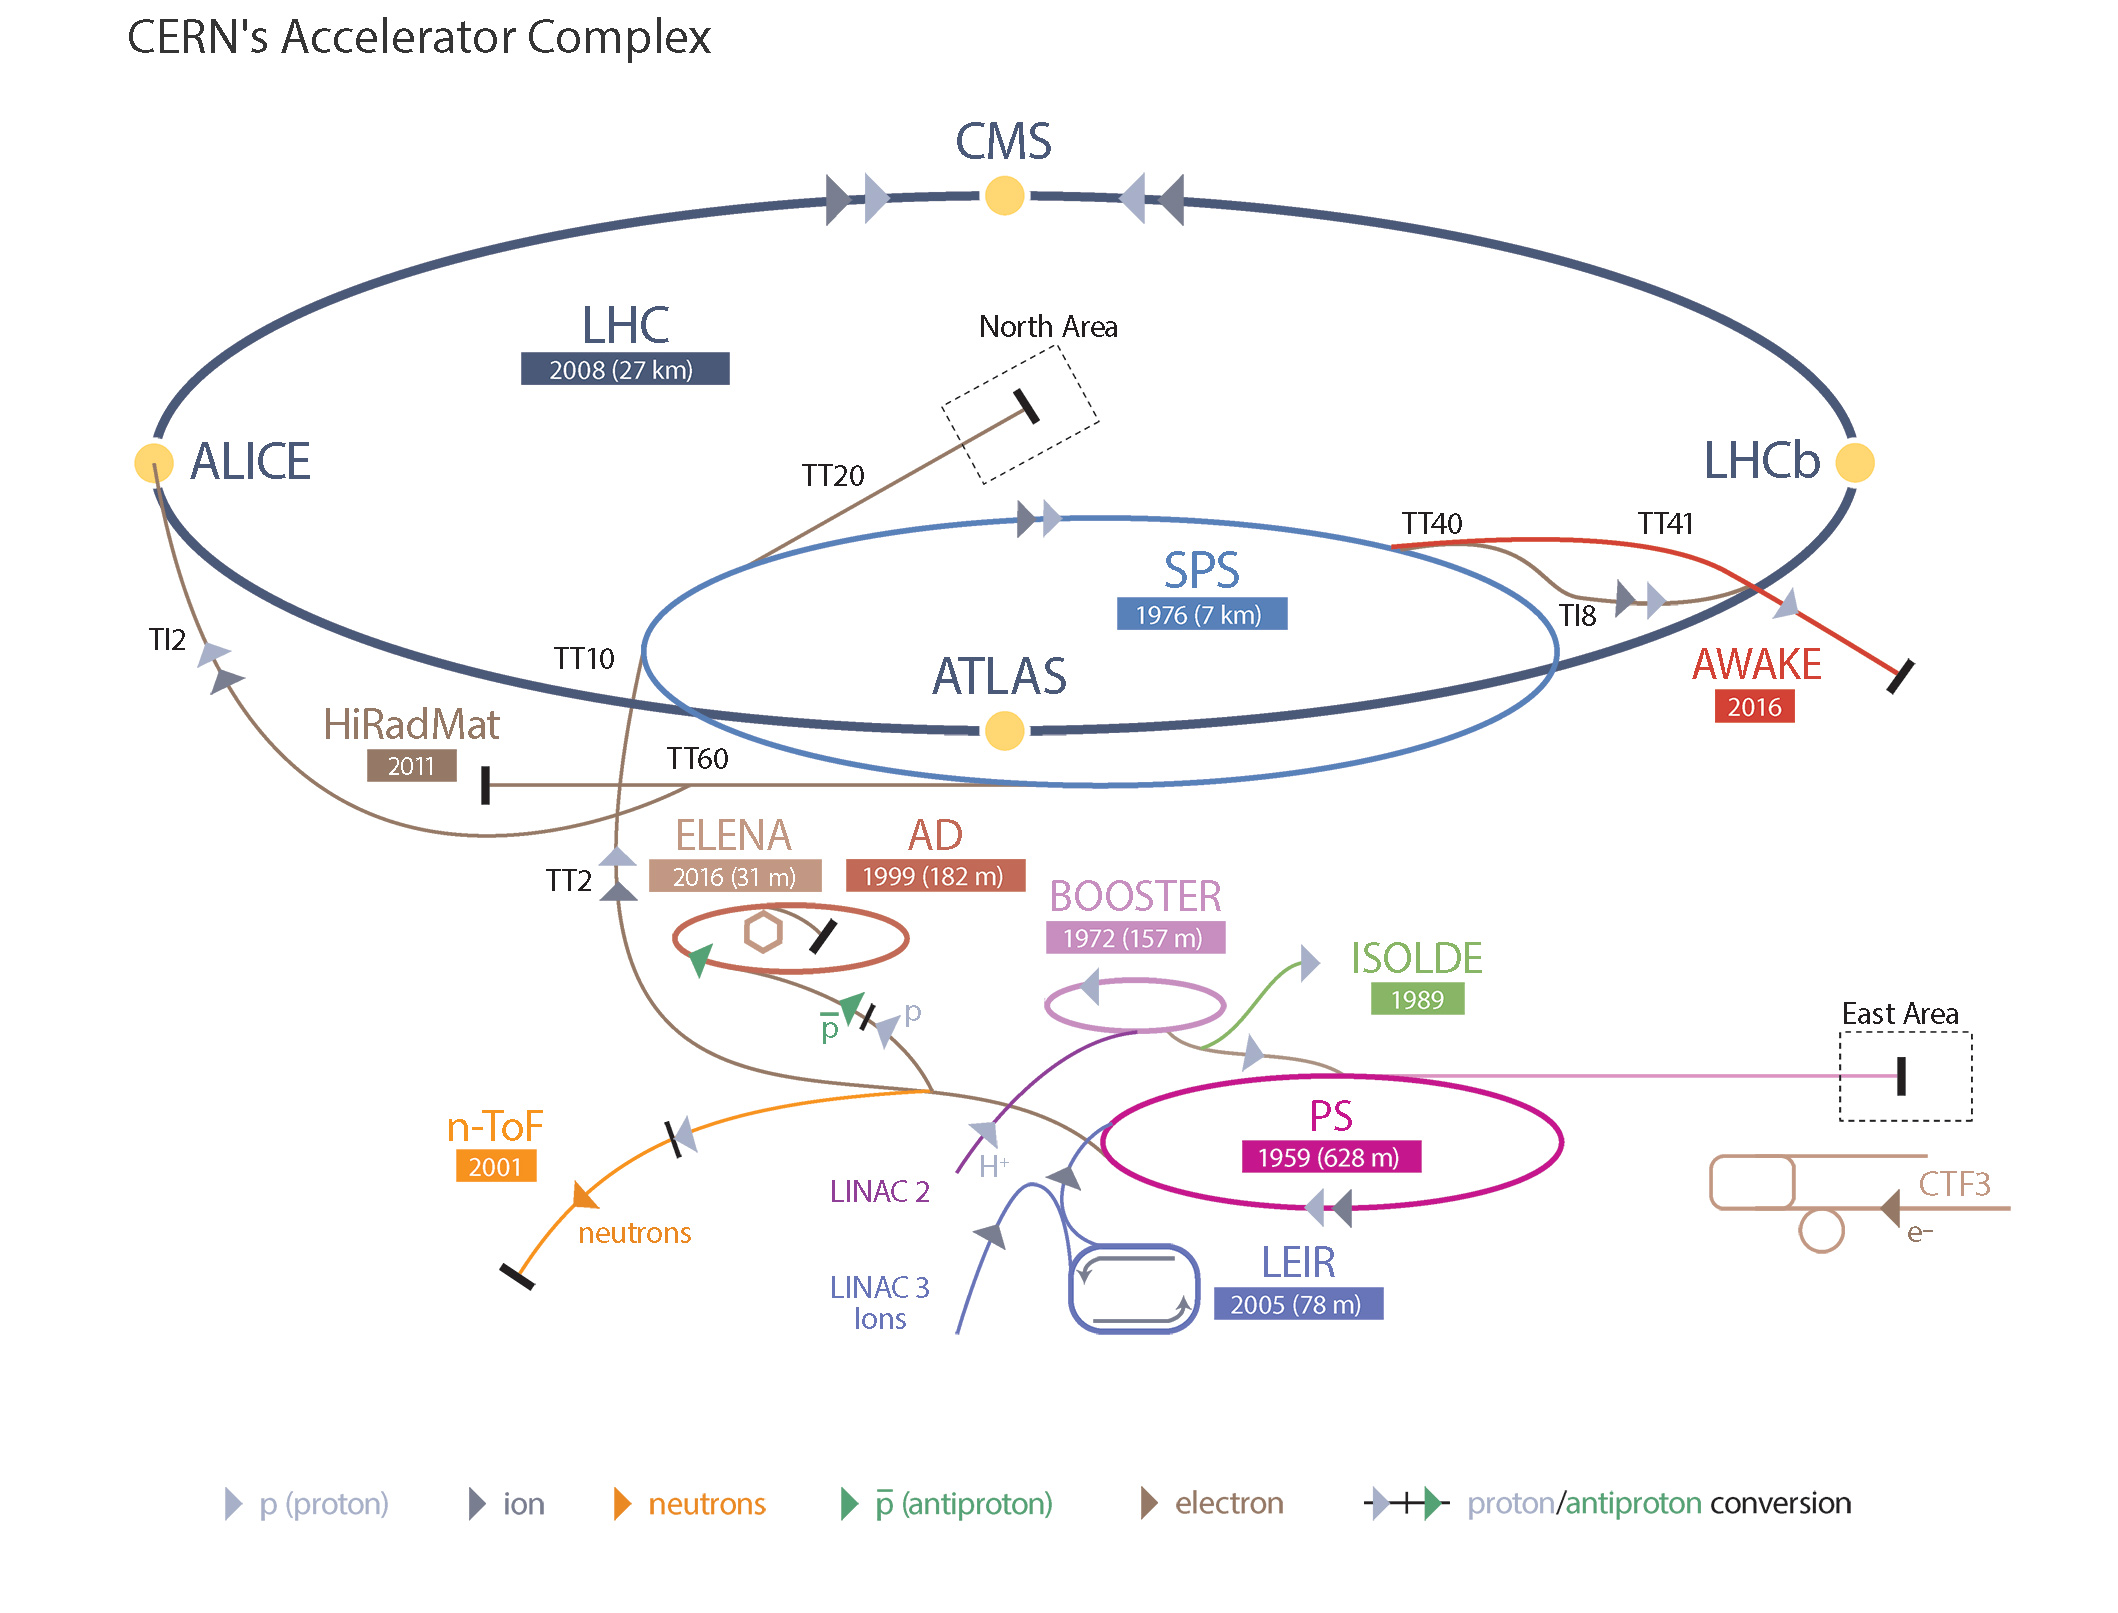
\includegraphics[width=17cm]{assets/chap02/lhc.jpg}
    \caption{The accelerator complex at CERN in Switzerland and France. Source: \cite{Marcastel:1621583}}
\end{figure}

The LHC operation consists so far of two runs: in run 1 in 2010, the first collisions at a center-of-mass energy of $\sqrt{s}=\SI{3.5}{TeV}$ started. The center-of-mass energy was upgraded in 2012 to $\sqrt{s}=\SI{8}{TeV}$. After a shutdown from 2013 to 2015, Run 2 began in 2015 at $\sqrt{s}=\SI{13}{TeV}$. The LHC will shut down by the end of 2018 to enter Run 3 at $\sqrt{s}=\SI{14}{TeV}$ in 2021.

Each of the four interaction point hosts one or multiple experiments. The most important ones are:
\begin{itemize}
\item \textbf{ATLAS} - A Toroidal LHC Apparatus
\item \textbf{CMS} - Compact Muon Solenoid
\item \textbf{ALICE} - A Large Ion Collider Experiment
\item \textbf{LHCb} - Large Hadron Collider beauty
\end{itemize}

The performance of a particle accelerator is quantified by the luminosity, which expresses the ratio between the event rate $\dv{N}{t}$ to the interaction cross-section $\sigma$ (the probability of a process to occur):
\begin{equation*}
    L=\frac{1}{\sigma} \dv{N}{t}
\end{equation*}
The larger the luminosity, the more likely an event of interest is to happen within a period of time.

\section{The Compact Muon Solenoid (CMS) Experiment}
\begin{figure}[!b]
    \centering
    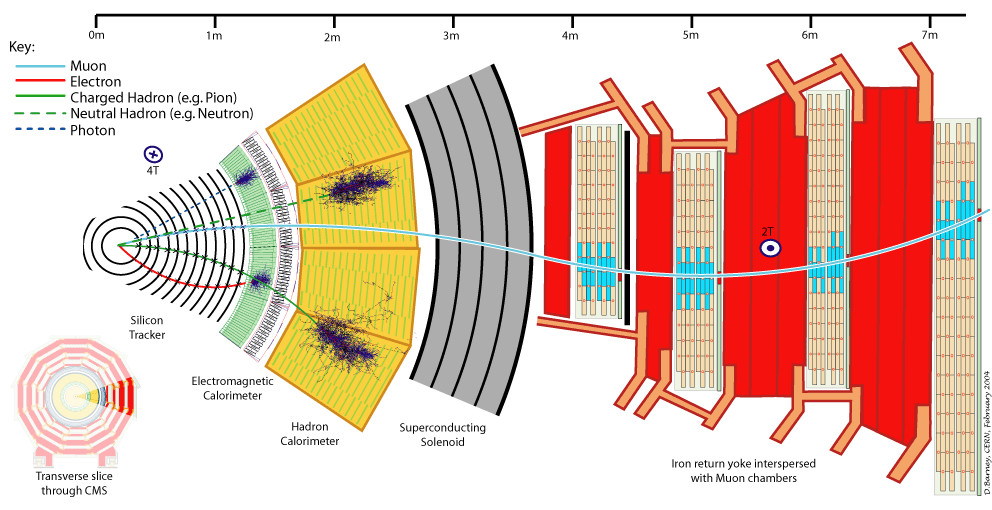
\includegraphics[width=15cm]{assets/chap02/cms.jpeg}
    \caption{Cross section view of the CMS detector and its components. Source: \cite{Davis:2205172}}
    \label{fig:cms}
\end{figure}
The CMS is a general-purpose particle detector built into the LHC, situated in an underground cavern at Cessy, France, built with the goal of investigating a wide range of physics, such as TeV-scale physics, the properties of the Higgs boson, heavy ion collisions, physics beyond the SM (supersymmetry, extra dimensions) and more. It has a length of \SI{28.7}{m}, a diameter of \SI{15}{m} and a weight of approximately \SI{14000}{t}. Figure \ref{fig:cms} shows a cross section view of the CMS detector.

The detector takes its name after its relatively small size, its muon tracking ability and powerful solenoid magnet.

The CMS is cylindrically symmetric towards the beam axis with the interaction point centrally located. The coordinate system is oriented such that the z axis is in the direction of the beam, the polar angle $\theta$ is defined in the r-z plane with the pseudorapidity defined as $\eta=-\ln{\tan{(\theta / 2)}}$. The momentum component transverse to the beam direction, $p_{\text{T}}$, is derived from the x- and y-components, the transverse energy is defined as $E_{\text{T}}=E \sin{\theta}$ \cite{Spannagel2017}.

The inside of the detector is permeated by a \SI{3.8}{T} magnet field orthogonal to the beam axis, created by the solenoid magnet, which deflects all charged particles within the detector in a helical path.

The components of the CMS from the point of interaction to its extremities are as follow \cite{Bhler:48721}:
\begin{itemize}
    \item \textbf{The Silicon Tracker} is made of silicon pixels and microstrip detectors, that measure the paths of particles traveling outwards from the interaction point. As they pass through the tracker, charged particles create electrons and holes in the semiconducting material, which lead to tiny electric signals that are amplified and detected. The charge and momentum of the particle can be inferred from the curvature of the reconstructed path. The tracker is limited to detecting only particles with $|\eta|<2.5$. One design goal for the tracker was to reduce the interactions of the particles with the tracker material to avoid distortions in momentum measurements.
    \item \textbf{The Electromagnetic Calorimeter} measures the energy of photons, electrons, and positrons by fully absorbing them. Lead tungstate crystals are used, which, due to the absorption, move to an excited state. The crystal leaves the excited state when photons are emitted. The intensity of the scintillation light is proportional to the energy of the absorbed particle and can be measured using photodetectors.
    \item \textbf{The Hadronic Calorimeter} measures the energy of hadrons, i.e. protons, neutrons, pions, and kaons. It is made of alternating layers of absorber material and plastic scintillators. The incoming particles create a cascade of secondary particles within the absorber that cause the scintillators to emit light.
    \item \textbf{The muon detectors} detect and reconstruct the paths of muons, similar to the silicon tracker. The muon detectors are located outside the solenoid. Due to their large mass compared to electrons, muons pass the inner components of the detector with negligible energy loss.
\end{itemize}

The CMS detector can not detect neutrinos, since they barely interact with matter. This is done indirectly exploiting momentum conservation, where the sum of the transverse momenta of the collision products must vanish. The transverse momentum of the neutrinos thus equals the negative sum of the transverse momenta of the detected collision products. Assuming the neutrinos are massless, their transverse momenta equals their energy. This is also known as missing transverse energy (MET):
\begin{equation*}
\slashed{E}_T=|-\sum{\va{p_T}}|
\end{equation*}